\chapter{Geometria/Relações (3º Bimestre)}

\section{Semelhança}

Da Wikipédia, duas figuras são semelhantes se elas possuem a mesma
forma, ou se uma das formas é a imagem espelhada da outra. Mais precisamente,
podemos obter uma das figuras ao realizar as seguintes operações na outra
figura: escala uniforme (aumentar ou reduzir), transladar, rotacionar ou
refletir.

Dois polígonos são semelhantes se

\begin{enumerate}
  \item Eles possuem o mesmo número de lados.
  \item Todos os lados encontram-se na mesma proporção.
  \item Os ângulos interiores são iguais.
\end{enumerate}

\subsection{Exercício 1}

Indique se os pares de figura a seguir são semelhantes ou apresente um
contra exemplo:

\begin{enumerate}
  \item Dois triângulos.
  \item Dois triângulos isósceles.
  \item Dois triângulos equiláteros.
  \item Dois quadrados.
  \item Dois retângulos.
  \item Dois losangos.
  \item Dois polígonos regulares convexos com o mesmo número de lados.
  \item Dois círculos.
  \item Duas elipses.
\end{enumerate}

\subsection{Exercício 2}

Considere os pontos cartesianos
$A=(1,0)$, $B=(3,0)$, $C=(0,3)$,
$D=(2,3)$, $E=(3,3)$, $F=(0,4)$, $G=(1,4)$, $H=(2,4)$ e $I=(3,4)$.
Indique se as formas a seguir são semelhantes:

\begin{enumerate}
\item $ABD$ e $DIG$
\item $ADG$ e $BDI$
\item $CDHF$ e $ABIG$
\item $EIG$ e $AIG$
\item $ABI$ e $CFG$
\end{enumerate}

Pode ser demonstrado que dois triângulos são semelhantes e uma das condições a
seguir for satisfeita:

\begin{enumerate}
  \item Todos os ângulos correspondentes são congruentes.
  \item Todos os lados correspondentes possuem comprimento na mesma proporção.
\item Dois lados possuem comprimento com a mesma proporção e o ângulo entre
  esses lados é igual.
\end{enumerate}

\subsection{Exercício 3}

Seja dois triângulos $ABC$ e $DEF$.

\begin{enumerate}
\item Mostre que
  se $\widehat{A} = \widehat{D}, \widehat{B} = \widehat{E}$
  então os triângulos são semelhantes.
\item O que pode ser afirmado se temos apenas $\widehat{A} = \widehat{D}$?
\item E se só temos $\frac{DE}{AB} = \frac{EF}{BC}$?
\end{enumerate}

\subsection{Exercício 4 (prova do Teorema de Pitágoras)}

Seja $ABC$ um triângulo retângulo em $C$. Seja $H$ a intersecção da hipotenusa
$A$ com a altura $C$. Seja $\alpha = \widehat{CAB}$
e $\beta=\widehat{ABC}$.

\begin{enumerate}
\item Determine os ângulos $\widehat{BCA}$, 
  $\widehat{BCH}$, $\widehat{ACH}$, $\widehat{CHA}$ e $\widehat{CHB}$
  em função de $\alpha, \beta$.
\item Mostre que
  $\frac{BC}{AB} = \frac{BH}{BC}$ e
  $\frac{AC}{AB} = \frac{AH}{AC}$.
\item Encontre o valor para ${BC}^2 + {AC}^2$.
\end{enumerate}

\section{Funciones trigonométricas}

\subsection{Definição}

Considere um triângulo retângulo e $\alpha$ a medida de um ângulo
em radianos ($0 \leq \alpha < \frac{\pi}{2}$).

\begin{center}
 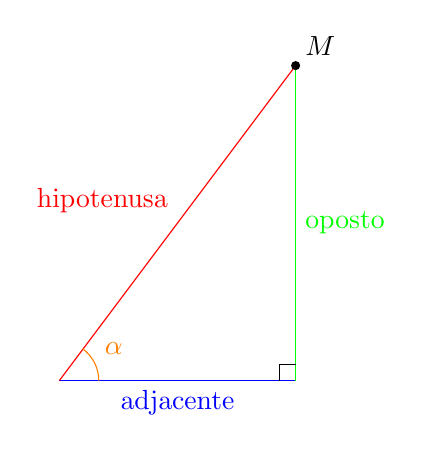
\begin{tikzpicture}
   \draw[color=blue] (0,0) -- (1.5,0)node[below]{adjacente} -- (3,0);
   \draw[color=green] (3,0) -- (3,2)node[right]{oposto} -- (3,4);
   \draw[color=red] (3,4) -- (1.5,2)node[above left]{hipotenusa} -- (0,0);
   \draw (2.8,0) -- (2.8,.2) -- (3,.2);
   \draw[color=orange] (0.5,0) arc(0:25:.5) node[above right]{$\alpha$}
   arc(25:53.13010235415599:.5);
   \draw[fill=black] (3,4) node[above right]{$M$} circle(.05);
 \end{tikzpicture}
\end{center}

Esses ângulos retos e $\alpha$ determinam a classe de semelhança do triângulo
e, portanto, as seguintes frações:

$$
\sin \alpha = \frac{\color{green}{\text{oposto}}}
{\text{\color{red}{\text{hipotenusa}}}}
$$
%%
$$
\cos \alpha = \frac{\color{blue}{\text{adjacente}}}
{\text{\color{red}{\text{hipotenusa}}}}
$$
%%
$$
\tan \alpha = \frac{\color{green}{\text{oposto}}}
{\text{\color{blue}{\text{adjacente}}}}
$$

Quando $\alpha$ se aproxima do ângulo reto, $\frac{\pi}{2}$,
o comprimento do lado oposto se aproxima da hipotenusa e
o comprimento do lado adjacente de aproxima de 0. Portanto, temos
%%
$$
\cos \frac{\pi}{2} = 0
$$
%%
$$
\sin \frac{\pi}{2} = 1
$$
%%
mas não definimos $\tan$ em $\frac{\pi}{2}$, porque a fração
pero no definimos $\tan$ en $\frac{\pi}{2}$, porque el cociente
$\frac{\color{green}{\text{oposto}}}
{\text{\color{blue}{\text{adjacente}}}}$ fica cada vez maior
quando $\alpha$ se aproxima de $\frac{\pi}{2}$.

Podemos generalizar as fórmulas anteriores se utilizarmos valores relativos para
$\color{green}{\text{oposto}}$ e ${\text{\color{blue}{\text{adjacente}}}}$
de acordo com a coordenada do vértice $M$ oposto ao ângulo $\alpha$:

$$\cos{(-\alpha)} = \cos{(\alpha)}$$
$$\sin{(-\alpha)} = -\sin{(\alpha)}$$
$$\tan{(-\alpha)} = -\tan{(\alpha)}$$
$$\cos{(\pi-\alpha)} = -\cos{(\alpha)}$$
$$\sin{(\pi-\alpha)} = \sin{(\alpha)}$$
$$\tan{(\pi-\alpha)} = -\tan{(\alpha)}$$

Finalmente ao completar uma volta $2\pi$ as frações devem ser a mesma e portanto
as funções devem ser periódicas:

$$\cos{(\alpha+2\pi)} = \cos{(\alpha)}$$
$$\sin{(\alpha+2\pi)} = \sin{(\alpha)}$$
$$\tan{(\alpha+2\pi)} = \tan{(\alpha)}$$

Essas fórmulas definem as funções seno e cosseno para todo
$\alpha \in \mathbb R$ e a função tangente para todo
$\alpha \in \left]{-\frac{\pi}{2} + k\pi}, {\frac{\pi}{2} +k\pi} \right[$
para $k \in \mathbb Z$. 

\subsection{Exercício 5}

\begin{enumerate}
  \item Qual é o seno, cosseno e tangente de $\alpha = 0$?
  \item Determine o ângulo $\alpha$ em um triângulo retângulo isosceles
    e depois o seno, cosseno e tangente de $\alpha$.
  \item Considere um triângulo equilátero $ABC$ e seja $D$ o ponto médio
    de $[BC]$. Mostre que $ABD$ é retângulo em $D$ e determine os
    ângulos $\widehat{A}$ e $\widehat{B}$
    bem como o seno, cosseno e tangente dos ângulos.
  \item Expresse o seno, cosseno e tangente dos ângulos
    $\frac{\pi}{6}$ e $\frac{\pi}{4}$ bem como de seus múltiplos.
\end{enumerate}

\subsection{Exercício 6}

Mostre as igualdades seguintes para
 $0 \leq \alpha < \frac{\pi}{2}$:

\begin{enumerate}
\item Utilize $\alpha + \pi = -\left(\pi-\alpha\right) + 2\pi$ para determinar
  $\cos\left(\alpha+\pi\right)$ e $\sin\left(\alpha+\pi\right)$.
\item $\tan \alpha = \frac{\sin \alpha}{\cos \alpha}$. Deduza que 
  $\tan \left(\alpha+\pi\right)$.
\item $\left(\sin \alpha\right)^2 + \left(\cos \alpha\right)^2 = 1$
\end{enumerate}

\subsection{Exercício 7}

\begin{enumerate}
\item Determine $\cos \frac{4\pi}{5}$ (respectivamente $\sin \frac{4\pi}{5}$)
  em função de $\cos \frac{\pi}{5}$ (respectivamente $\sin \frac{\pi}{5}$)
  utilizando a fórmulas do cosseno (respectivamente seno) para
  $\pi - \alpha$.
\item Na figura seguinte, determine todos os ângulos e comprimentos além de
  deduzir as fórmulas:

$$
{\sin {2\alpha}} = {2 {\sin \alpha} {\cos \alpha}}
$$
%%
$$
{\cos {2\alpha}} = {2 \left(\cos \alpha\right)^2 - 1}
$$

\begin{center}
 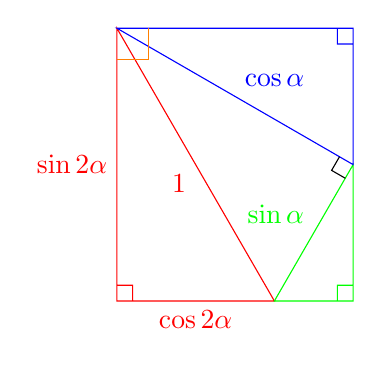
\begin{tikzpicture}
   \draw[color=red] (0,0) -- (1,0)node[below]{$\cos {2\alpha}$} --  (2,0) --
   (1,1.732050807568877)node[below left]{$1$} --
   (0,3.464101615137754) -- (0,1.732050807568877)node[left]{$\sin {2\alpha}$} --
   cycle (.2,0) -- (.2,.2) -- (0,.2);
   \draw[color=green] (2,0) -- (3,0) -- (3,1.732050807568877) -- 
   (2.5,0.86602540378443)node[above left]{$\sin \alpha$} -- cycle
   (2.8,0) -- (2.8,.2) -- (3,.2);

   \draw[color=blue] (3,1.732050807568877) -- (3,3.464101615137754) --
   (0,3.464101615137754) -- 
   (1.5,2.598076211353315)node[above right]{$\cos \alpha$} -- cycle
   (2.8,3.464101615137754) -- (2.8,3.264101615137754) -- (3,3.264101615137754);
   \draw[color=orange]
   (.4,3.464101615137754) -- (.4,3.064101615137754) -- (0,3.064101615137754);
   \begin{scope}[rotate around={-30:(3,1.732050807568877)}]
   \draw (2.8,1.732050807568877) -- (2.8,1.532050807568877) --
   (3,1.532050807568877);
   \end{scope}
 \end{tikzpicture}
\end{center}

\item Sjea $x = \cos \frac{\pi}{5}$. Temos $0 < x < 1$.
 Utilize as fórmulas da pergunta anterior para mostrar
%%
$$
{\sin \left(\frac{4\pi}{5}\right)} = 4 x \left(2x^2-1\right) \sin\left(\frac{\pi}{5}\right)
$$
%%
$$
{\cos \left(\frac{4\pi}{5}\right)} = 2 \left(2x^2 - 1\right)^2 - 1
$$

\item Mostre que $4x^2 - 2x -1 = 0$ e deduza
  $$
  {\cos \left(\frac{2\pi}{5}\right)} = \frac{\sqrt{5}-1}{4}
  $$
\item
  Use o exercícoo 8 de BraFuMat7 (construir uma raiz quadrada) para desenhar um
  pentágono de raio $4$.

\end{enumerate}

\section{Solução de problemas envolvendo triângulos rectângulos}

\subsection{Definição}

Se fixarmos a longitude da hipotenusa e movermos o ponto $M$ para a parte
do plano tal que $0 \leq \alpha < \frac{\pi}{2}$,
os limites dos lados oposto e adjacente são:

$$0 \leq {\color{green}{\text{oposto}}} \leq {\color{red}{\text{hipotenusa}}}$$
$$0 \leq {\color{blue}{\text{adjacente}}} \leq {\color{red}{\text{hipotenusa}}}$$

\begin{center}
 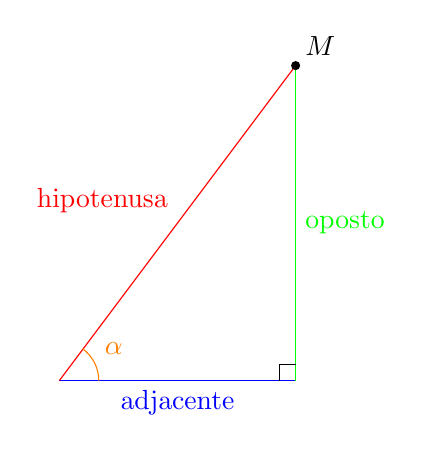
\begin{tikzpicture}
   \draw[color=blue] (0,0) -- (1.5,0)node[below]{adjacente} -- (3,0);
   \draw[color=green] (3,0) -- (3,2)node[right]{oposto} -- (3,4);
   \draw[color=red] (3,4) -- (1.5,2)node[above left]{hipotenusa} -- (0,0);
   \draw (2.8,0) -- (2.8,.2) -- (3,.2);
   \draw[color=orange] (0.5,0) arc(0:25:.5) node[above right]{$\alpha$}
   arc(25:53.13010235415599:.5);
   \draw[fill=black] (3,4) node[above right]{$M$} circle(.05);
 \end{tikzpicture}
\end{center}

e então
%%
$$
0\leq \sin \alpha \leq 1
$$
$$
0\leq \cos \alpha \leq 1
$$

Reciprocamente um número real $0 \leq x \leq 1$ determina um único triângulo
retângulo
${\color{blue}{\text{adjacente}}} = x$,
${\color{green}{\text{oposto}}} = \sqrt{1-x^2}$ e
${\color{red}{\text{hipotenusa}}} = 1$ e então um único ângulo
$0 \leq \alpha_1 \leq \frac{\pi}{2}$. Definimos
%%
$$
\alpha_1 = \arccos x
$$

Da mesma forma, um número real $0 \leq x \leq 1$ determina um único triângulo
retângulo
${\color{green}{\text{oposto}}} = x$,
${\color{blue}{\text{adjacente}}} = \sqrt{1-x^2}$ e
${\color{red}{\text{hipotenusa}}} = 1$ e então um único ângulo
$0 \leq \alpha_2 \leq \frac{\pi}{2}$. Definimos
%%
$$
\alpha_2 = \arcsin x
$$

Agora fixamos a longitude do lado adjacente e movemos o ponto $M$ para a parte
do plano tal que
$0 \leq \alpha < \frac{\pi}{2}$. $M$ pode mover-se
verticalmente e o comprimento de
${\color{green}{\text{oposto}}}$ pode ir de $0$ a um
valor tão grande quanto quisermos. Um real $x \geq 0$, determina um
único triângulo ${\color{green}{\text{oposto}}} = x$,
${\color{blue}{\text{adjacente}}} = 1$ e
${\color{red}{\text{hipotenusa}}} = \sqrt{1+x^2}$ e portanto um único
ângulo $0 \leq \alpha_3 < \frac{\pi}{2}$. Definimos
%%
$$
\alpha_3 = \arctan x
$$

As funções seno, cosseno, tangente, arco cosseno, arco seno, arco tangente
estão disponíveis em calculadoras (científicas) o que permite resolver problemas
envolvendo triângulos retângulos quando conhecemos dois parâmetros (lado ou
ângulo não reto).

\subsection{Exercício 8}

Seja $ABC$ um triângulo retângulo em $A$. Determine uma aproximação para

\begin{enumerate}
\item a longitude $BC$ se $\widehat{C} = 15°$ e $AC = 10\text{cm}$.
\item a amplitude do ângulo $\widehat{B}$ se $AC = 5\text{cm}$ e
  $BC = 8\text{cm}$.
\item a amplitude de $AB$ se $AC = 8\text{cm}$ e $\widehat{B} = 65°$.
\item a longitude $AB$ se $BC = 15\text{cm}$ e $\widehat{B} = 55°$.
\end{enumerate}

\section{Solução dos Exercício}

\subsection{Exercício 1}

\begin{enumerate}
  \item Não. Considere um triângulo retângulo e um triângulo equilátero.
  \item Não. Considere um triângulo equilátero e um triângulo isosceles com um
    lado maior do que o outro.
  \item Sim.
  \item Sim.
  \item Não. Considere um quadrado e um retângulo com a largura maior que a altura.
  \item Não. Considere um quadrado e um losango cujos ângulos não são retos.
  \item Sim.
  \item Sim.
  \item Não. Considere um círculo e uma elipse como semi-eixo maior e semi-eixo
    menor não são iguais.
\end{enumerate}

\subsection{Exercício 2}

\begin{enumerate}
  \item Não.
  \item Sim.
  \item Sim.
  \item Sim.
  \item Não.
\end{enumerate}

\subsection{Exercício 3}

\begin{enumerate}
\item Temos
  $\widehat{C} = {180° - \widehat{A} - \widehat{B}} =
  {180° - \widehat{D} - \widehat{E}} = \widehat{F}$ e então
  os triângulos são semelhantes.
\item É fácil encontrar dois triângulos com $\widehat{A} = \widehat{D}$
  mas com outro ângulo que não correspondente.
\item Considerar por exemplo $A = D$, $B = E$ e $AB = AC = DF$ mas
  $90° = \widehat{A} \neq \widehat{D} = 135°$.
\end{enumerate}

\subsection{Exercício 4 (Prova do Teorema de Pitágoras)}

\begin{enumerate}
\item Temos três triângulos retângulos e
$\widehat{BCA} = \widehat{CHA} = \widehat{CHB} = 90°$. Entã
  $\widehat{BCH} = 90° - \beta = \alpha$ e
  $\widehat{ACH} = 90° - \alpha = \beta$.
\item Os triângulos $ABC$ e $ACH$ possuem ângulos congruentes e portanto são
  similares. Os lados correspondentes possuem comprimento na mesma proporção
  e portanto $\frac{AC}{AB} = \frac{AH}{AC}$.
  De forma semelhante, podemos mostrar que
  $BAC$ e $BCH$ são similares e que $\frac{BC}{AB} = \frac{BH}{BC}$.
\item A igualdade anterior fornece que ${AC}^2 = {AH} \times {AB}$
  e ${BC}^2 = {BH} \times {AB}$. Deduzimos então que
  ${BC}^2 + {AC}^2 = \left({AH} + {BH}\right) \times {AB} = {AB}^2$.
\end{enumerate}

\subsection{Exercício 5}

\begin{enumerate}
\item Quando $\alpha=0$, ${\color{green}{\text{oposto}}} = 0$ e
  ${\color{blue}{\text{adjacente}}} = \text{\color{red}{\text{hipotenusa}}}$
  então ${\tan 0} = {\sin 0} = 0$ y $\cos 0 = 1$.
\item Para um triângulo retângulo isósceles,
  $\frac{\pi}{2} + \alpha + \alpha = \pi$
  então $\alpha = \frac{\pi}{4} = 45°$.
  Se $x$ é o comprimento de um dos catetos,
  temos ${\color{green}{\text{oposto}}} = {\color{blue}{\text{adjacente}}} = x$
  e pelo Teorema de Pitágoras
  $\text{\color{red}{\text{hipotenusa}}} = x \sqrt{2} $.
  Então $\sin \frac{\pi}{4} = \cos \frac{\pi}{4} = \frac{x}{x \sqrt{2}} = \frac{\sqrt{2}}{2}$
  e $\tan \frac{\pi}{4} = 1$.
\item Seja $x$ o comprimento de um dos lados do triângulo retângulo equilátero
  $ABC$: ${AB} = {AC} = {BC} = x$.
  $D$ é o ponto médio de $[BC]$ então ${AD} = \frac{BC}{2} = \frac{x}{2}$.
  Além disso, por que $A, D$ encontram-se sobre a mediatriz de $[BC]$ e
  $ABD$ é retângulo em $D$ (que é o mesmo que $\widehat{D} = \frac{\pi}{2}$).
  Pelo Teorema de Pitágoras,
  $AD = \sqrt{x^2 - \left(\frac{x}{2}\right)^2} = \frac{\sqrt{3}}{2} x$.
  $ABC$ é equilátero e portanto $\widehat{B} = \frac{\pi}{3} = 60°$ e
  $\widehat{A} = \pi - \widehat{D} - \widehat{B} = \frac{\pi}{6}$.
  Finalmente, 
  $\sin \widehat{A} = \cos \widehat{B} = \frac{x/2}{x} = \frac{1}{2}$
  $\cos \widehat{A} = \sin \widehat{B} = \frac{\frac{\sqrt{3}}{2} x}{x} =
  \frac{\sqrt{3}}{2}$,
  $\tan \widehat{A} = \frac{\sqrt{3}}{3}$ e
  $\tan \widehat{B} = \sqrt{3}$.
\item Já obtemos os valores para
  $\alpha = 0, \frac{\pi}{6}, \frac{\pi}{4}, \frac{\pi}{3}, \frac{\pi}{2}$.
  Utilizando a simetria das funções trigonométricas,
  podemos deduzir os valore para os múltiplos desses ângulos.

  \begin{center}
  \begin{tabular}{| l | c | c | c | c | c | c | c | c | c | c | c | c | c | c | c | c |}
    \hline
    $\alpha$ &
    $-\frac{5\pi}{6}$ &
    $-\frac{3\pi}{4}$ &
    $-\frac{2\pi}{3}$ &
    $-\frac{\pi}{2}$ &
    $-\frac{\pi}{3}$ &
    $-\frac{\pi}{4}$ &
    $-\frac{\pi}{6}$ &
    $0$ &
    $\frac{\pi}{6}$ &
    $\frac{\pi}{4}$ &
    $\frac{\pi}{3}$ &
    $\frac{\pi}{2}$ &
    $\frac{2\pi}{3}$ &
    $\frac{3\pi}{4}$ &
    $\frac{5\pi}{6}$ &
    $\pi$ \\
    \hline
    $\sin \alpha$ & 
    $-\frac{1}{2}$ &
    $-\frac{\sqrt{2}}{2}$ &
    $-\frac{\sqrt{3}}{2}$ &
    $-1$ &
    $-\frac{\sqrt{3}}{2}$ &
    $-\frac{\sqrt{2}}{2}$ &
    $-\frac{1}{2}$ &
    $0$ &
    $\frac{1}{2}$ &
    $\frac{\sqrt{2}}{2}$ &
    $\frac{\sqrt{3}}{2}$ &
    $1$ &
    $\frac{\sqrt{3}}{2}$ &
    $\frac{\sqrt{2}}{2}$ &
    $\frac{1}{2}$ &
    $0$
    \\
    \hline
    $\cos \alpha$ &
    $-\frac{\sqrt{3}}{2}$ &
    $-\frac{\sqrt{2}}{2}$ &
    $-\frac{1}{2}$ &
    $0$ &
    $\frac{1}{2}$ &
    $\frac{\sqrt{2}}{2}$ &
    $\frac{\sqrt{3}}{2}$ &
    $1$ &
    $\frac{\sqrt{3}}{2}$ &
    $\frac{\sqrt{2}}{2}$ &
    $\frac{1}{2}$ &
    $0$ &
    $-\frac{1}{2}$ &
    $-\frac{\sqrt{2}}{2}$ &
    $-\frac{\sqrt{3}}{2}$ &
    $-1$
    \\
    \hline
    $\tan \alpha$ & 
    $\frac{\sqrt{3}}{3}$ &
    $1$ &
    $\sqrt{3}$ &
    / &
    $-\sqrt{3}$ &
    $-1$ &
    $-\frac{\sqrt{3}}{3}$ &
    $0$ &
    $\frac{\sqrt{3}}{3}$ &
    $1$ &
    $\sqrt{3}$ &
    / &
    $-\sqrt{3}$ &
    $-1$ &
    $-\frac{\sqrt{3}}{3}$ &
    $0$
    \\
    \hline
  \end{tabular}
  \end{center}
  
\end{enumerate}

\subsection{Exercício 6}

\begin{enumerate}
\item $\cos \left(\alpha + \pi\right) =
  \cos \left(-\left(\pi-\alpha\right) + 2\pi\right) = 
  \cos \left(-\left(\pi-\alpha\right)\right) =
  \cos \left(\left(\pi-\alpha\right)\right) = -\cos(\alpha)$ e

$\sin \left(\alpha + \pi\right) =
  \sin \left(-\left(\pi-\alpha\right) + 2\pi\right) = 
  \sin \left(-\left(\pi-\alpha\right)\right) =
  -\sin \left(\left(\pi-\alpha\right)\right) = -\sin(\alpha)$
\item $\frac{\sin \alpha}{\cos \alpha} =
\frac{\frac{\color{green}{\text{oposto}}}{\text{\color{red}{\text{hipotenusa}}}}}{\frac{\color{blue}{\text{adjacente}}}{\text{\color{red}{\text{hipotenusa}}}}} = 
\frac{\color{green}{\text{oposto}}}{\color{blue}{\text{adjacente}}} =
{\tan \alpha}$. Então, 
$\tan \left(\alpha+\pi\right) = \frac{-\sin \alpha}{-\cos \alpha} =
\frac{\sin \alpha}{\cos \alpha} = {\tan \alpha}$.

\item $\left(\sin \alpha\right)^2 + \left(\cos \alpha\right)^2 = 
  \frac{{\color{green}{\text{oposto}}}^2
    +{\color{blue}{\text{adjacente}}}^2
    }{\text{\color{red}{\text{hipotenusa}}}^2} = 1$ pelo Teorema de Pitágoras.
\end{enumerate}

\subsection{Exercício 7}

\begin{enumerate}
\item
  $$\cos\left(\frac{4\pi}{5}\right) = \cos\left(\pi-\frac{\pi}{5}\right) =
  -\cos\left(-\frac{\pi}{5}\right) = -\cos\left(\frac{\pi}{5}\right)$$
  $$\sin\left(\frac{4\pi}{5}\right) = \sin\left(\pi-\frac{\pi}{5}\right) =
  -\sin\left(-\frac{\pi}{5}\right) = \sin\left(\frac{\pi}{5}\right)$$

\item No triângulo retângulo roxo, o ângulo adjacente ao lado de comprimento
  $\cos 2\alpha$ mede $2\alpha$ e o ângulo oposto $\frac{\pi}{2} - 2\alpha$.
  Da mesma maneira, no triângulo retângulo central, o ângulo adjacente
  ao lado de longitude $\cos \alpha$ mede $\alpha$ e o ângulo posto
  $\frac{\pi}{2} - \alpha$. Portanto, encontramos os ângulos que tocam
  esses ângulos no triângulo retângulo azul ($\frac{\pi}{2} -
  \left(\frac{\pi}{2} - 2\alpha\right) - \alpha =
  \alpha$) e verde ($\pi - 2\alpha - \left(\frac{\pi}{2}-\alpha\right) =
  \frac{\pi}{2} - \alpha$).
  Finalmente, obtemos os ângulos que tocam o ângulo reto do triângulo central:
  $\frac{\pi}{2} - \alpha$ (triângulo azul) e $\alpha$
  (triângulo verde) e podemos verificar que somam 180° com o ângulo reto
  do triângulo central.

  Os lados do triângulo azul são $\left(\cos \alpha\right)^2$ (horizontal) e
  ${\sin \alpha} {\cos \alpha}$ (vertical). 
  Os lados do triângulo verde são $\left(\sin \alpha\right)^2$ (horizontal) e
  ${\sin \alpha} {\cos \alpha}$ (vertical). Finalmente,
%%
  $${\sin \left(2\alpha\right)} = 2 {\sin \alpha} {\cos \alpha}$$
%%
  $${\cos \left(2\alpha\right)} = \left(\cos \alpha\right)^2 - 
  \left(\sin \alpha\right)^2 = 
  2\left(\cos \alpha\right)^2 - 1$$
  
  Deste modo, utilizando a fórmula do exercício 5 para simplicar
  $\cos \left(2\alpha\right)$.

\item 

${\sin \left(\frac{4\pi}{5}\right)} = 2 {\sin \left(\frac{2\pi}{5}\right)}
{\cos \left(\frac{2\pi}{5}\right)}$ e
${\cos \left(\frac{4\pi}{5}\right)} =
2 \left({\cos \left(\frac{2\pi}{5}\right)}\right)^2 - 1$. Além disso,
${\sin \left(\frac{2\pi}{5}\right)} = 2 x {\sin \left(\frac{\pi}{5}\right)}$ e
${\cos \left(\frac{2\pi}{5}\right)} = 2x^2 - 1$.

\item Porque
$\sin\left(\frac{4\pi}{5}\right) = \sin\left(\frac{\pi}{5}\right) \neq 0$,
a primeira igualdade torna-se
%%
$$2 \left(2x^2-1\right) = \frac{1}{2x}$$

E porque $\cos\left(\frac{4\pi}{5}\right) = -\cos\left(\frac{\pi}{5}\right) = -x$
a segunda igualdade torna-se
%%
$$2\left(2x^2-1\right)^2 = 1 - x$$

Se tomamos o quociente da segunda pela primeira, obteremos
%%
$$
2x^2 - 1 = {2x\left(1 - x \right)} = 2x - 2x^2
$$
%%
e então
%%
$$
4x^2 - 2x - 1 = 0
$$

A solução positiva dessa equação é
$x = \frac{2 + \sqrt{4+16}}{8} = \frac{1+\sqrt{5}}{4}$
e finalmente
%%
  $$
  {\cos \left(\frac{2\pi}{5}\right)} = {2x^2 - 1} = \frac{\sqrt{5}-1}{4}
  $$

\item Para desenhar o pentágono regular de raio $4$,
  é suficiente determinar
  $4 {\cos \left(\frac{2\pi}{5}\right)} = \sqrt{5} - 1$.
  Mas $\sqrt{5}$ pode ser obtido utilizando a construção
  do exercício 8 de BraFuMat7.
  Finalmente obtemos o esquema a seguir que pode ser desenhado
  utilizando régua e compasso:

\begin{center}
\begin{tikzpicture}
  \draw (0,0) circle(4)[color=blue];
  \draw[fill=black] (0,0) circle(.05)[color=blue];
  \draw (-5,0) -- (5,0)[dashed,color=red];
  \draw (0,-5) -- (0,5)[dashed,color=red];
  \draw[fill=black] (2.23606797749979,0) circle(.05);
  \draw[dashed, color=magenta]
  (0,0) -- (0,-.4) -- (0.6,-.4)
  node[below]{$4 \cos\left(\frac{2\pi}{5}\right)$} --
  (1.23606797749979, -.4) -- (1.23606797749979, 0);
  \draw[dashed, color=orange] (2.23606797749979,0) -- (2.23606797749979,-.2) --
  (1.78606797749979,-.2) node[below]{$1$} -- (1.23606797749979,-.2) --
  (1.23606797749979,0);
  \draw[fill=black] (1.23606797749979,0) circle(.05);
  \draw[color=green](0,0) -- (1.23606797749979, 0) -- 
  (1.23606797749979,3.804226065180614) --
  (.6, 1.9)node[above left]{$4$} -- (0,0);
  \draw[color=green] (1.23606797749979, 0) -- (4,0) -- 
  (1.23606797749979,3.804226065180614);
  \draw[color=green](1.43606797749979,0) --
  (1.43606797749979,.2) -- (1.23606797749979,.2);
  \draw[color=green]
  (1.23606797749979,3.804226065180614) --
  (-3.236067977499789,2.351141009169893) --
  (-3.23606797749979,-2.351141009169892) --
  (1.23606797749979,-3.804226065180614) -- (4, 0);
  \draw[color=cyan](0,.4) -- (1.118033988749895,.4) node[above]{$\sqrt{5}$} --
  (2.23606797749979,.4);

\end{tikzpicture}
\end{center}

\end{enumerate}

\subsection{Exercício 8}

\begin{enumerate}
\item $BC = \frac{AC}{\cos 15°} \approx 10.36\text{cm}$.
\item $\widehat{B} = \arcsin \frac{5}{8} \approx 38°41'$
\item $AB = \frac{AC}{\tan 65°} \approx 18.93\text{cm}$.
\item $AB = BC {\cos 55°} \approx 8.60\text{cm}$.
\end{enumerate}
